\chapter{Image Fusion}
\section{Guided Image Filter 2013}
\subsection{Abstract}
In this paper, we propose a novel explicit image filter called guided filter. Derived from a local linear model, the guided filter
computes the filtering output by considering the content of a guidance image, which can be the input image itself or another different
image. The guided filter can be used as an edge-preserving smoothing operator like the popular bilateral filter, but it has better
behaviors near edges. The guided filter is also a more generic concept beyond smoothing: It can transfer the structures of the guidance
image to the filtering output, enabling new filtering applications like dehazing and guided feathering. Moreover, the guided filter
naturally has a fast and nonapproximate linear time algorithm, regardless of the kernel size and the intensity range. Currently, it is one
of the fastest edge-preserving filters. Experiments show that the guided filter is both effective and efficient in a great variety of
computer vision and computer graphics applications, including edge-aware smoothing, detail enhancement, HDR compression, image
matting/feathering, dehazing, joint upsampling, etc.
\subsection{Content}
A general linear translation-variant filtering process, which involves a guidance image \textit{I}, an filtering input image \textit{p} and an output image \textit{q}. Both \textit{I} and \textit{p} are given beforehand according to the application, and they can be \textbf{identical}! The filtering output at a pixel \textit{i} is expressed as a weight average:
\begin{equation}
\centering
q_i = \sum_{j}W_{ij}(I)p_j
\end{equation}
where \textit{i, j} are pixel indexes. The filter kernel \(W_{ij}\) is a function of the guidance image \textit{I} and independent of \textit{p}.
\subsection{Conclusion}

\section{Multiscale Image Fusion Through Guided Filtering}
\subsection{Abstract}
We introduce a multiscale image fusion scheme based on GUided Filtering. Guided filtering can effectively reduce noise while preserving details boundaries. While  restoring larger scale edges. The proposed multi-scale fusion scheme achieves optimal spatial consistency by using guided filtering both at the decomposing and at the recombination stage of the multiscale fusion process. First, size-selective iterative guided filtering is applied to decompose the source images into base and detail layers at multiple levels of resolution. Next, at each resolution level a binary weighting map is obtained as the pixelwise maximum of
corresponding source saliency maps. Guided filtering of the binary weighting maps with their corresponding source images as guidance images serves to reduce noise and to restore spatial consistency. The final fused image is obtained as the weighted recombination of the individual detail layers and the mean of the lowest resolution base layers. Application to multiband visual (intensified) and thermal infrared imagery demonstrates that the proposed method obtains state-of-the-art performance for the fusion of multispectral nightvision images. The method has a simple implementation and is computationally efficient\cite{toet2016multiscale}.

\subsection{Contents}
To data, a variety of image fusion algorithms have been proposed. A popular class of algorithms are the multi-scale image fusion schemes, which decompose the source images into spatial primitives at multiple spatial scales, then integrate these primitives to form a new multi-scale transform-based representation, and finally apply an inverse multi-scale transform to reconstruct the fused image. However, most of these techniques are computationally expensive and tend to oversharpen edges, which makes them less suitable for application in multiscale schemes

Bilateral Filter: It can reverse the intensity gradient near sharp edges.

Guided Filter: 

The two filtering conditions are:
\begin{itemize}
\item the local filter output is a linear transform of the guidance image \textit{G}
\item as similar as possible to the input image \textit{I}.
\end{itemize}
The first condition implies that:
\begin{displaymath}
O_i = a_kG_i + b_k \qquad \forall i \in \omega_k
\end{displaymath}
where the $\omega_k$ is a square window of size $(2r + 1) \times (2r+1)$. {\bfseries The local linear model ensures that the output image $O$ has an edge only at locations where the guidance image $G$ also has one.} Linear coefficients $a_k$ and $b_k$ are constant in $\omega_k$. They can be estimated by minimizing the squared difference between the output image $O$ and the input image $I$ in the window $\omega_k$, i.e. minimizing the cost function $E$:
\begin{displaymath}
E(a_k, b_k) = \sum_{i \in \omega_k}\left((a_kG_i + b_k - I_i)^2 + \epsilon a_k^2 \right)
\end{displaymath}
where $\epsilon_k$ is a regularization parameter penalizing large $a_k$. The coefficients $a_k$ and $b_k$ can directly be solved by linear regression. Since pixel $i$ is contained in several different window $\omega_k$, the value of $O_i$ depends on the window over which it is calculated:
\begin{displaymath}
O_I = \overline{a}_i G_i + \overline{b}_i
\end{displaymath}
The abrupt intensity changes in the guiding image $G$ are still largely preserved in the output image $O$. The guided filter is a computationally efficient, edge-preserving operator which avoids the gradient reversal artefacts of the bilateral filter. 

In Iterative guided filtering: In such a scheme the result $G^{t+1}$ of the t-\textit{th} iteration is obtained from the joint bilateral filtering of the input image $I$ using the result $G^t$ of the previous iteration step:
\begin{displaymath}
G^{t+1}_i = \frac{1}{K_i}\sum_{j \in \omega}I_j \cdot f(\parallel i - j \parallel) \cdot g(\parallel G^t_i - G^t_j \parallel )
\end{displaymath}
Note that the initial guidance image $G^1$ can simply be a constant (e.g. zero) valued image since it updates to the Gaussian filtered input image in the first iteration step.

Proposed Method:
\begin{itemize}
\item Iterative guided filtering is applied to decompose the source images into base layers (representing large scale variations) and detail layers (containing small scale variations).
\item Frequency-tuned filtering is used to generate saliency maps for the source images.
\item Binary weighting maps are computed as the pixelwise maximum of the individual source saliency maps.
\item Guided filtering is applied to each binary weighting map with its corresponding source as the guidance image to reduce noise and to restore spatial consistency.
\item The fused image is computed as a weighted recombination of the individual source detail layers.
\end{itemize}

\textbf{Visual saliency} refers to the physical, bottom-up distinctness of image details. It is a relative property that depends on the degree to which a detail is visually distinct from its background. {\bfseries \color{red} Since saliency quantifies the relative visual importance of image details saliency maps are frequently used in the weighted recombination phase of multiscale image fusion schemes}. Frequency tuned filtering computes bottom-up saliency as local multiscale luminance contrast. The saliency map S for an image I is computed as 
\begin{displaymath}
S(x, y) = \parallel I_\mu - I_f(x,y) \parallel 
\end{displaymath}
where\\
\indent $I_\mu$ is the arithmetic mean image feature vector\\
\indent $I_f$ represents a Gaussian blurred version of the original image, using a 5 * 5 separable binomial kernel\\
\indent $\parallel \cdot \parallel $ is the $L_2$ norm(Euclidian distance), and x, y are the pixel coordinates.\\
\indent We compute saliency using frequency tuned filtering since a recent and extensive evaluation study comparing 13 state-of-the-art saliency models found that the output of this simple saliency model correlates more strongly with human visual perception than the output produced by any of the other available models.

Binary weight maps $BW_{X_i}$ and $BW_{Y_i}$ are then computed by taking the pixelwise maximum of corresponding saliency maps $S_{X_i}$ and $S_{Y_i}$:

\begin{gather*}
BW_{X_i}(x, y) =    
\begin{cases}
1 & \mathrm{if} \: S_{X_i}(x, y) > S_{Y_i}(x, y) \\
0 & \mathrm{otherwise}
\end{cases}\\
BW_{Y_i}(x,y) = 
\begin{cases}
1 & \mathrm{if} \: S_{Y_i}(x, y) > S_{X_i}(x, y)\\
0 & \mathrm{otherwise}
\end{cases}
\end{gather*}
The resulting binary weight maps are noisy and typically not well aligned with object boundaries, which may give rise to artefacts in the final fused image. Spatial consistency is therefore restored through guided filtering (GF) of these binary
weight maps with the corresponding source layers as guidance images
\begin{gather*}
W_{X_i} = GF(BW_{X_i}, X_i) \\
W_{Y_i} = GF(BW_{Y_i}, Y_i)
\end{gather*}

Fused detail layers are then computed as the normalized weighted mean of the corresponding source detail layers:
\begin{displaymath}
dF_i = \frac{W_{X_i} \cdot dX_i + W_{Y_i} \cdot dY_i}{W_{X_i} + W_{Y_i}}
\end{displaymath}

The fused image $F$ is finally obtained by adding the fused detail layers to the average value of the lowest resolution source layers:
\begin{displaymath}
F = \frac{X_3 + Y_3}{2} + \sum_{i=0}^{2}dF_i
\end{displaymath}

By using guided filtering both in the decomposition stage and in the recombination stage, this proposed fusion scheme optimally benefits from both the multi-scale edge-preserving characteristics (in the iterative framework) and the structure
restoring capabilities (through guidance by the original source images) of the guided filter. The method is easy to implement and computationally efficient.

\subsection{Conclusion}
We propose a multiscale image fusion scheme based on guided filtering. Iterative guided filtering is used to decompose the source images into base and detail layers. Initial binary weighting maps are computed as the pixelwise maximum of
the individual source saliency maps, obtained from frequency tuned filtering. Spatially consistent and smooth weighting maps are then obtained through guided filtering of the binary weighting maps with their corresponding source layers as
guidance images. Saliency weighted recombination of the individual source detail layers and the mean of the lowest resolution source layers finally yields the fused image. The proposed multi-scale image fusion scheme achieves spatial consistency by using guided filtering both at the decomposition and at the recombination stage of the multiscale fusion process. Application to multiband visual (intensified) and thermal infrared imagery demonstrates that the proposed method obtains state-of-the-art performance for the fusion of multispectral nightvision images. The method has a simple implementation and is computationally efficient.

\section{Image Fusion With Guided Filtering}
\subsection{Abstract}
A fast and effective image fusion method is proposed for creating a highly informative fused image through merging multiple images. The proposed method is based on a two-scale decomposition of an image into a base layer containing large scale variations in intensity, and a detail layer capturing small scale details. A novel guided filtering-based weighted average technique is proposed to make full use of spatial consistency for fusion of the base and detail layers. Experimental results
demonstrate that the proposed method can obtain state-of-the-art performance for fusion of multispectral, multifocus, multimodal, and multiexposure images.
\subsection{Contents}
\subsubsection{Guided Filter}
The filtering output $O$ is linear transformation of the guidance image $I$ in a local window $\omega_k$ centered at pixel $k$:
\begin{displaymath}
O_i = a_k I_i + b_k \qquad \forall i \in \omega_k
\end{displaymath}
where $\omega_k$ is a square window of size $(2r+1) \times (2r+1)$. The linear coefficients $a_k$ and $b_k$ are contant in $\omega_k$ by minimizing the squared difference between the output image $O$ and the input iamge $P$:
\begin{displaymath}
E(a_k, b_k) = \sum_{i \in \omega_k}\left( (a_kI_i + b_k - P_i) + \epsilon a_k^2 \right)
\end{displaymath}
where $\epsilon$ is a regularization parameter given by the user.
The coefficients can be directly solved by linear regression as follows:
\begin{gather*}
a_k = \frac{\frac{1}{|\omega|}\sum_{i \in \omega_k}I_iP_i -  \mu_k \overline{P}_k}{\delta_k + \epsilon}
\\
b_k = \overline{P}_k - a_k \mu_k
\end{gather*}
where $\mu_k$ and $\delta_k$ are the mean and variance of $I$ in $\omega_k$ respectively. $|\omega|$ is the number of pixels in $\omega_k$, and $\overline{P}_k$ is the mean of $P$ in $\omega_k$. Then the output image can be calculated according to above equation.
\begin{displaymath}
O_i = \overline{a}_iI_i + \overline{b}_i
\end{displaymath}
where \(\overline{a}_i = \frac{1}{|\omega|}\sum_{k \in \omega_i}a_k, \overline{b}_i = \frac{1}{|\omega|}\sum_{k \in \omega_i}b_k \). 

The color image situation, the $a_i$ and other calculators become vector version. See \cite{li2013image}.

\subsection{Fusion Frame}
See figure \ref{fig2.1}.
\begin{figure}[!hbpt]
\centering
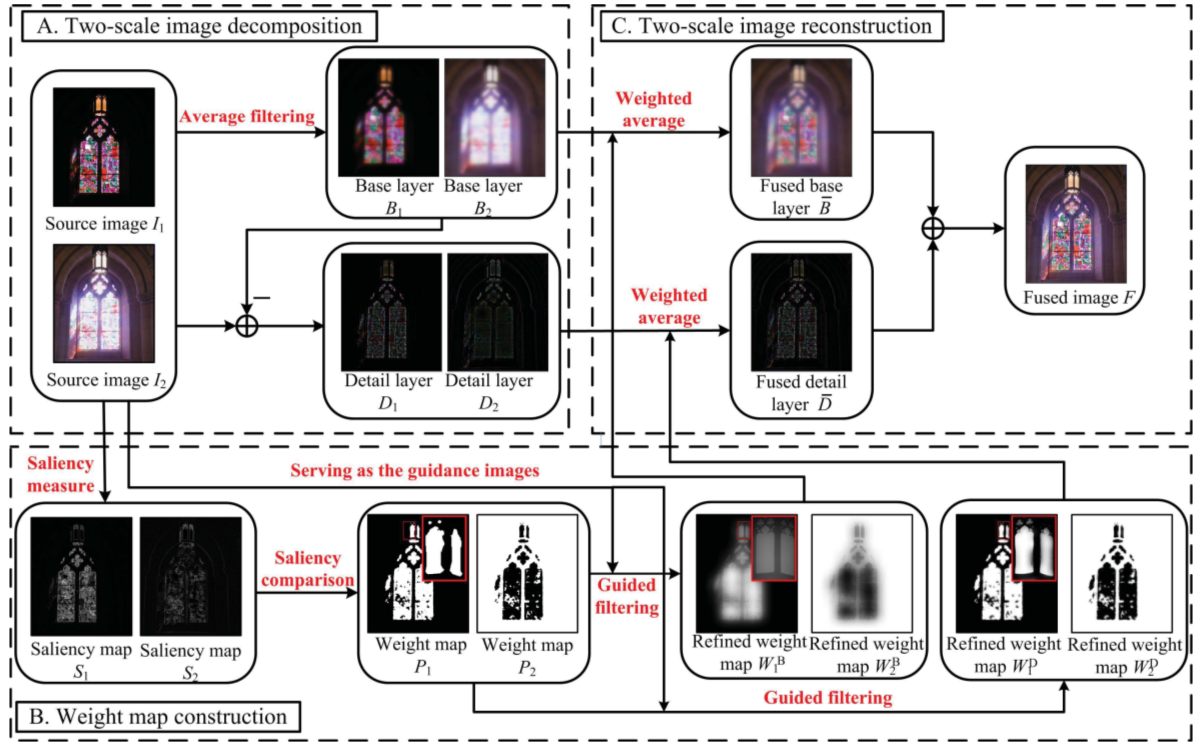
\includegraphics[width=0.9\textwidth]{ImageFusion/ImageFusionGuidedFilter1}
\caption{Schematic diagram of the proposed image fusion method based on guided filtering.}
\label{fig2.1}
\end{figure}

\subsection{Conclusion}